\documentclass[lettersize,journal]{IEEEtran}
\usepackage{amsmath,amsfonts}
\usepackage{algorithmic}
\usepackage{algorithm}
\usepackage{array}
\usepackage[caption=false,font=normalsize,labelfont=sf,textfont=sf]{subfig}
\usepackage{textcomp}
\usepackage{stfloats}
\usepackage{url}
\usepackage{verbatim}
\usepackage{graphicx}
\usepackage{cite}
\hyphenation{op-tical net-works semi-conduc-tor IEEE-Xplore}
% updated with editorial comments 8/9/2021

% \usepackage{amsmath,amsfonts}
% \usepackage{algorithmic}
% \usepackage{array}
% \usepackage[caption=false,font=normalsize,labelfont=sf,textfont=sf]{subfig}
% \usepackage{cite}
% \usepackage{textcomp}
% \usepackage{stfloats}
% \usepackage{url}
% \usepackage{verbatim}
% \usepackage{graphicx}
\usepackage{amssymb}
\usepackage{xcolor}
% \usepackage{appendix}
% \usepackage{algorithm}
\usepackage{amsthm}
% \usepackage{multirow} 
% \usepackage{multicol} 
% \usepackage{color}
\usepackage{bm}
% \hyphenation{op-tical net-works semi-conduc-tor IEEE-Xplore}
\usepackage{hyperref}
\usepackage{scalerel}
\usepackage{float}%提供float浮动环境
\usepackage{booktabs}%提供命令\toprule、\midrule、\bottomrule
\newtheoremstyle{custom}
  {\topsep}    % 上方间距
  {\topsep}    % 下方间距
  {\normalfont} % 定理内容的字体 (普通字体)
  {1em}           % 缩进量
  {\itshape}   % 定理标题的字体 (斜体)
  {:}          % 标题后的标点符号
  { }          % 标题后与内容的间距
  {\thmname{\textit{#1}}% 定理标题格式 (斜体)
   \thmnumber{ \textit{#2}}% 定理编号格式 (斜体)
   \thmnote{ \textit{(#3)}}}% 定理备注格式 (斜体)
% 应用自定义样式
\theoremstyle{custom}
\newtheorem{Thm}{Theorem}
\newtheorem{Lem}{Lemma}
\newtheorem{Cor}{Corollary}
\newtheorem{Def}{Definition}
\newtheorem{Exam}{Example}
\newtheorem{Alg}{Algorithm}
\newtheorem{Prob}{Problem}
\newtheorem{subproblem}{Problem}[Prob]
\newtheorem{Rem}{Remark}
\newcommand{\RNum}[1]{\uppercase\expandafter{\romannumeral #1\relax}}
\newcommand{\tabincell}[2]{\begin{tabular}{@{}#1@{}}#2\end{tabular}}
% \theoremseparator{:}
\newtheorem{hyp}{Hypothesis}

\begin{document}

\title{A Novel Action-Relevance-Aware Multi-View Token Allocation Approach for Wireless VLA Inference}

\author{IEEE Publication Technology,~\IEEEmembership{Staff,~IEEE,}
        % <-this % stops a space
\thanks{This work was supported by the National Natural Science Foundation of China under Grant 62571307, the Science and Technology Commission Foundation of Shanghai under Grants 24DP1500703, 24DP1500500, and the National Key Research and Development Program of China under Grants 2022YFB2902304. (Corresponding author: Shunqing Zhang. )}% <-this % stops a space
\thanks{Zaiyu Jin, Jihong Li and Shunqing Zhang are with the School of Communication and Information Engineering, Shanghai University, Shanghai, 200444, China (e-mail: 18321125576@163.com, tomlijiong@shu.edu.cn, shunqing@shu.edu.cn). }}

% The paper headers
\markboth{Journal of \LaTeX\ Class Files,~Vol.~14, No.~8, August~2021}%
{Shell \MakeLowercase{\textit{et al.}}: A Sample Article Using IEEEtran.cls for IEEE Journals}

\IEEEpubid{0000--0000/00\$00.00~\copyright~2021 IEEE}
% Remember, if you use this you must call \IEEEpubidadjcol in the second
% column for its text to clear the IEEEpubid mark.

\maketitle

\begin{abstract}
Deploying vision-language-action (VLA) models in wireless embodied
systems requires multi-view visual information to be transmitted under
stringent bandwidth and latency constraints. Although existing
visual-token pruning methods can reduce inference costs, they generally
operate under predetermined token budgets and overlook heterogeneous
wireless transmission conditions across sensing views. To address this
limitation, we propose an action-relevance-aware multi-view token
allocation framework for wireless edge VLA inference. The framework
characterizes the marginal contribution of retained visual tokens to
VLA action preservation through a dataset-calibrated action-utility
model. It then jointly allocates view-specific token budgets according
to predicted action relevance and instantaneous wireless transmission
costs. To ensure causal operation, current action relevance is estimated
from delayed feedback, and a generalized water-filling method with
integer correction is developed to obtain feasible token allocations.
Experiments with GR00T-N1.6-3B on the RoboCasa
\emph{PnPSinkToCounter} task show that the proposed method adapts
effectively to time-varying relevance and channel conditions. Using
full-token inference as the action reference, it achieves
52.3\%--79.3\% lower normalized action mean-square error than BestCQI
across the evaluated SNR range and a 26.1\% average reduction compared
with random feasible allocation. These results demonstrate that jointly
exploiting action relevance and wireless channel conditions enables more
effective use of limited communication resources for edge VLA
inference.
\end{abstract}

\begin{IEEEkeywords}
Edge VLA inference, multi-view token pruning, relevance-aware communication, wireless resource allocation
\end{IEEEkeywords}

\section{Introduction}
\IEEEPARstart{V}{ision}-Language-Action (VLA) models have emerged as a promising paradigm for embodied intelligence by integrating visual perception, language understanding, and action generation into a unified inference pipeline. Their deployment, however, is particularly challenging in wireless embodied systems, where multiple heterogeneous sensing nodes continuously observe the environment and the resulting sensory information must be delivered under stringent latency and bandwidth constraints. Wireless networked robotic and cyber-physical systems have therefore increasingly emphasized the joint design of sensing, communication, computing, and control rather than optimizing each component independently \cite{fang2025sc3,pang2025codesign,diao2025taskoriented}. In this paper, we focus on the communication bottleneck created by visual tokens: each sensing node locally extracts visual tokens, retains only a task-relevant subset, and transmits the retained tokens to an edge VLA for action inference.

A first line of related work attempts to reduce the substantial inference cost of VLA models. EfficientVLA jointly removes redundant language layers, prunes task-aware visual tokens, and reuses diffusion features \cite{yang2025efficientvla}; SP-VLA jointly exploits temporal action redundancy through model scheduling and spatial redundancy through spatio-semantic token pruning \cite{li2025spvla}; and DySL-VLA dynamically skips incremental layers according to action importance \cite{yang2026dyslvla}. Complementary model-compression approaches further reduce memory and arithmetic overhead. QVLA explicitly measures channel-wise action-space sensitivity for mixed-precision quantization \cite{xu2026qvla}, QuantVLA develops scale-calibrated post-training quantization for VLA backbones and action heads \cite{zhang2026quantvla}, and DyQ-VLA adapts bit widths according to temporally varying action sensitivity \cite{zheng2026dyqvla}. These approaches substantially improve on-device or edge-side computational efficiency, but their optimization targets are primarily compute, memory, or fixed compression budgets rather than heterogeneous wireless transmission resources.

Visual-token pruning provides a particularly relevant mechanism for reducing both computation and communication load. EfficientVLA selects compact task-aware visual tokens \cite{yang2025efficientvla}, while VLA-Pruner reveals a semantic--action gap between vision-language prefill saliency and action-decode relevance and therefore combines semantic importance with temporally smoothed action relevance \cite{liu2026vlapruner}. SpecPrune-VLA exploits spatial-temporal consistency and combines action-level static pruning with layer-level dynamic pruning \cite{wang2026specprune}, whereas VLA-IAP preserves interaction-critical visual structures and dynamically adjusts pruning intensity according to semantic-motion alignment \cite{cheng2026vlaiap}. Recent work also studies the theoretical tradeoff among multiple visual-token selection objectives under a fixed budget \cite{li2026balancedcovering}. Nevertheless, these methods mainly answer \emph{which} tokens should be removed under a prescribed computational/token budget. They do not provide an analytical rule for \emph{how many} tokens each sensing node should transmit when wireless costs are heterogeneous, nor do they address that the VLA internal action-relevance signal is generated at the edge and is causally available to sensing nodes only after feedback delay.
\IEEEpubidadjcol

A second line of work studies communication--control co-design in wireless networked control systems (WNCSs). Han \emph{et al.} jointly optimize wireless resources while guaranteeing finite-time system-identification performance \cite{han2024wsi}, and further jointly optimize transmit power, transmission intervals, coding parameters, and reliability for energy-efficient WNCS operation \cite{han2026energy}. Fang \emph{et al.} formulate sensing--communication--computing--control loops for digital-twin-enabled robotic systems and derive closed-form or approximate resource-allocation structures for minimizing linear-quadratic-regulator cost \cite{fang2025sc3}. Pang \emph{et al.} address large-scale coupled WNCSs with time-correlated wireless channels through a scalable deep-reinforcement-learning codesign \cite{pang2025codesign}, while Wang \emph{et al.} jointly optimize transmission scheduling and mobile-agent movement under state-dependent fading with control-performance guarantees \cite{wang2025heterogeneous}. These studies establish rigorous links between communication resources and control objectives, but the model-based derivations are typically built on explicit plant/control models such as system identification, stochastic switched systems, or LQR-type costs. Such analytical mappings are unavailable for nonlinear VLA inference, whose action error depends on high-dimensional, interacting visual tokens.

Task-oriented and semantic communication offers another route to transmit only information relevant to downstream objectives. Diao \emph{et al.} co-design information-bottleneck-based task-oriented JSCC with delay-aware control prediction for edge-enabled industrial cyber-physical systems \cite{diao2025taskoriented}. Pan \emph{et al.} formulate hierarchical goal-oriented semantic errors for distributed sensing--communication--control systems and dynamically adapt sensor transmission rates using learned semantic compression and reinforcement learning \cite{pan2025semantic}. Wang \emph{et al.} derive task-oriented rate relationships under distortion, perception, and classification constraints \cite{wang2025lossy}, while Wu \emph{et al.} develop an information-theoretic multimodal bottleneck framework that dynamically balances task-relevant information across modalities \cite{wu2025omib}. Although these methods demonstrate the value of task-aware representation and rate allocation, they either rely on task-specific learned codecs/policies or analytical task models that differ fundamentally from a pre-trained VLA. Consequently, a tractable relationship between retained VLA token numbers and action error, together with a causal mechanism for exploiting delayed VLA internal relevance over wireless links, remains missing.

Motivated by the above gap, we study action-relevance-aware token allocation for wireless edge VLA inference. The key idea is to calibrate, for a fixed target dataset and sensing configuration, the expected marginal action-error reduction brought by additional retained tokens, and then use the resulting action-utility law to connect VLA internal relevance with wireless token allocation. Because the internal relevance is produced only after edge inference, the online allocation is made causal through one-slot-delayed relevance prediction. This enables the communication budget to be distributed across sensing nodes according to both embodied-task utility and instantaneous wireless transmission cost.

Motivated by these, our main contributions are summarized as follows: 
\begin{itemize}
    \item \textbf{Wireless-aware multi-sensor token allocation framework:}
    We formulate a wireless-enabled embodied AI framework in which multiple sensing nodes perform local visual-token pruning and transmit only the retained tokens to an edge VLA for action inference. 
    Different from existing VLA token-pruning methods that mainly optimize computational efficiency under fixed token budgets, we explicitly couple the per-sensor retained token numbers with heterogeneous wireless transmission costs and formulate the resulting action-error minimization problem under an air-interface bandwidth constraint.

    \item \textbf{Action-relevance model and delayed-feedback-aware token allocation:}
    To address the analytically intractable relationship between multi-sensor token pruning and nonlinear VLA action performance, we establish a calibrated marginal action-utility model that characterizes the expected action-error reduction as a function of the VLA internal action relevance and the retained token number of each sensor.
    Based on this model, the original action-error minimization problem is transformed into a tractable action-relevance-aware utility maximization problem.
    Moreover, considering that the VLA internal action-relevance signal is generated at the edge only after inference, we develop a causal allocation mechanism using delayed relevance feedback and derive a generalized water-filling solution that jointly accounts for task relevance, diminishing token utility, and wireless transmission cost.

    \item \textbf{Experimental validations:}  
    We implement the proposed scheme using the GR00T-N1.6-3B VLA model and evaluate it on the RoboCasa \emph{PnPSinkToCounter} task under time-varying wireless channels. The experimental results verify the rapid numerical convergence of the generalized water-filling solver and demonstrate that the proposed scheme can causally adapt the view-specific token budgets according to delayed action relevance and instantaneous channel conditions. Across the evaluated SNR range, the proposed scheme reduces the normalized action MSE by 52.3\%--79.3\% compared with the communication-only BestCQI baseline and by 26.1\% compared with random feasible allocation when aggregated over all evaluated SNR points. 

\end{itemize}
The remainder of this paper is organized as follows. Section~II introduces the system, communication, and token-compression models. Section~III formulates the original action-error minimization problem. Section~IV constructs a tractable problem transformation using dataset-calibrated marginal action utility and delayed action-relevance feedback. Section~V develops the online token-allocation algorithm, and Section~VI analyzes the resulting allocation rule and computational complexity. Section~VII presents the experimental results, followed by the conclusions.

\section{System Model}
\begin{figure*}
    \centering
    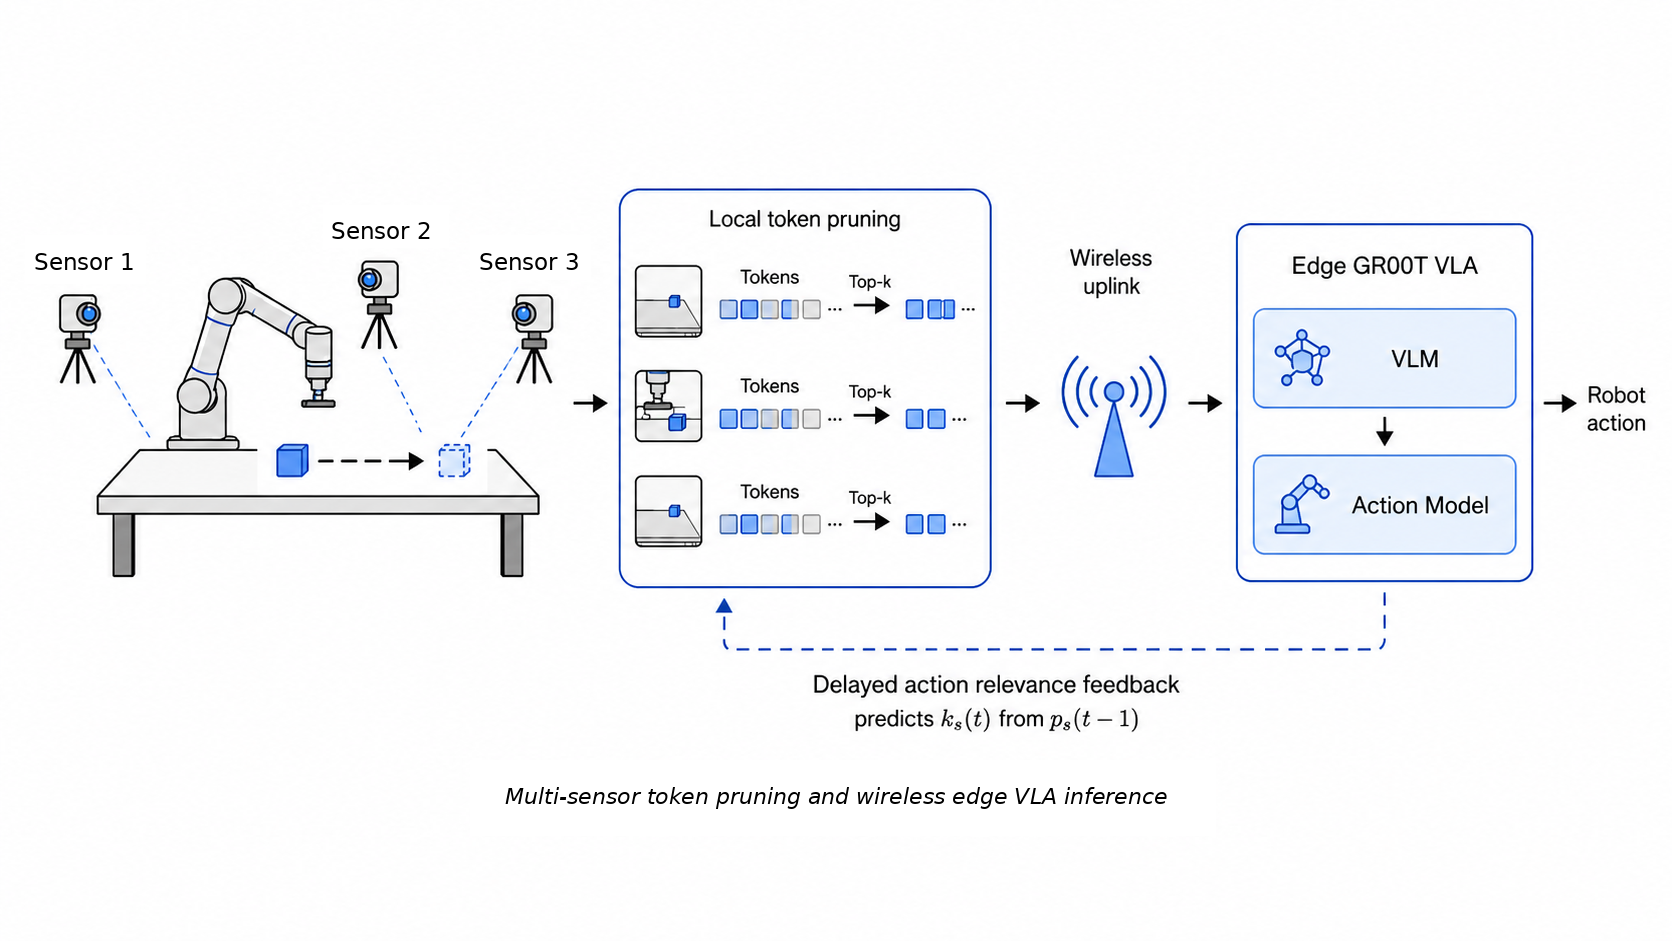
\includegraphics[
        width=\linewidth,
        trim=0 50 0 30,
        clip
    ]{system_model.png}
    \caption{System model.}
    \label{fig:system_model}
\end{figure*}
In this paper, we study a wireless-enabled embodied AI (WEEA) system, where an embodied agent and the corresponding sensing nodes $\mathcal{S} = \{1, \ldots, s, \ldots, S\}$ are connected to the edge remote controller $e$ with Vision-Language-Action (VLA) equipped. 
% $I$ agents with sensing and action abilities are distributed in the space. 
The system is illustrated in Fig.~\ref{fig:system_model}. Each sensing node perceives the environment with observations $\mathcal{V}_s(t) \in \mathcal{V}(t)$ (e.g., RGB images), its raw data volume is identified with $d_s(t)$. The edge VLA model receive $\mathcal{V}(t)$ and a time-invariant language instruction (prompt) $p$, then VLA model generate policy $\Pi_\theta(\mathcal{A}(t) \vert \mathcal{V}(t), p)$ to predict an action sequence $\mathcal{A}(t)$ (e.g., end-effector poses or joint velocities), where $\theta$ denotes the VLA model parameter. 
% singel-cell system where the base station (BS) is equipped with edge computing power, serving a set of user equipments (UEs), denoted by $i \in \mathcal{I}$. 
% Each agent contains hybrid content transmissions of multi-modal sensory data from helper agent $j$ to ego agent $i$, denoted with ${\bf d}_{j, i}(t) = \{ d^\mathrm{v}_{j, i}(t), d^\mathrm{r}_{j, i}(t), \ldots \}$, where $d^\mathrm{v}_{j, i}(t)$, $d^\mathrm{r}_{j, i}(t)$ represent the transmission data volume of vision, radar, etc., from helper agent $j$ to ego agent $i$, respectively. 
% Each agent contains hybrid content transmissions of multi-modal sensory data and control data, profiled with ${\bf q}_i(t) = \{ {\bf q}^\mathrm{v}_i(t), {\bf q}^\mathrm{r}_i(t), {\bf q}^\mathrm{ms}_i(t), \ldots , {\bf q}^\mathrm{mc}_i(t) \}$, where ${\bf q}^\mathrm{v}_i(t) = \{ {\bf d}^\mathrm{v}_i(t), f^\mathrm{v} \}$, ${\bf q}^\mathrm{r}_i(t) = \{ {\bf d}^\mathrm{r}_i(t), f^\mathrm{r} \}$, ${\bf q}^\mathrm{ms}_i(t) = \{ d^\mathrm{ms}_i(t), f^\mathrm{ms} \}$ and ${\bf q}^\mathrm{mc}_i(t) = \{ d^\mathrm{mc}_i(t), f^\mathrm{mc} \}$ represent the transmission profile of vision, radar, motor state and motor control for agent $i$, including data volume and transmission frequency, respectively. 


% \subsection{xxx Protocol Design}
% Identifying the multi-modal sensory feedback

% The communication resource grid is 



% Puncturing\footnote{xxx} and finite block-length short packet transmission are enabled for ultra low-latency high-reliability motor state and control signal transmissions. The puncturing duration at sub-channel $f$ is denoted by $t_{i, f} < T_k, i \in \mathcal{I}_{m}$. 
% % Puncturing\footnote{xxx} is enabled for ultra low-latency high-reliability transmissions, which is suitable for text queries transmissions carrying more semantic information within each bits \cite{}. 

\subsection{Communication Model}
The up-link transmission rate from sensing node $s$ to the edge server at slot $t$ is described as
\begin{align}
    r_{s}(t) = B_s(t) log_2\left(1 + \mathrm{SNR}_s(t) \right), \forall s \in \mathcal{S}, 
\end{align}
where $B_s(t)$ and $\mathrm{SNR}_s(t)$ denote the fractional bandwidth allocated to $s$ and the signal-to-noise ratio (SNR) of $s$, respectively. The fractional bandwidth allocation follows
\begin{align}\label{bandwidth_cons}
    \sum_{s \in \mathcal{S}}B_s(t) \leq B, 
\end{align}
where $B$ is the system bandwidth\footnote{We assume that adequate bandwidth $B$ is semi-persistently allocated to the WEEA system via orthogonal radio access network (RAN) slicing}. 

% The transmission rate from helper agent $j$ to ego agent $i$ at slot $t$ is described as: 
% \begin{align}
%     r_{j, i}(t, f) = B \sum_{f \in \mathcal{F}} b_{f, j, i}(t) \log_2\left(1 + \frac{p_{j, i}(t) h_{j, i}(t)}{\vartheta^2} \right), 
%     % i \in \mathcal{I}_i \cup \mathcal{I}_v &, 
% \end{align}
% % \begin{align}
% %     r_{n, i}(t, f) = (1 - \sum_{i \in \mathcal{I}_\mathrm{t}}\frac{t_{i, f}}{T_k})\log_2\left(1 + \frac{p_{n, i}(t) h_{n, i}(t)}{\vartheta^2} \right) &, \nonumber\\
% %     i \in \mathcal{I}_i \cup \mathcal{I}_v &, 
% % \end{align}
% where $h_{j, i}(t)$ is the channel coefficient from $j$ to $i$, $B$ is unit bandwidth of sub-channel, $\vartheta$ is the xxx and $b_{f, j, i}(t)$, $p_{j, i}(t)$ is the sub-channel allocation indicator and the transmit power, respectively. $b_{f, j, i}(t) = 1$ means sub-channel $f$ is allocated for the data transmission from $j$ to $i$ and $b_{f, j, i}(t) = 0$ otherwise.  The transmit power of each agent $i$ is bounded by 
% \begin{align}
%     \sum_{i \in \mathcal{I}, i \neq j} p_{j, i}(t) \leq P_\mathrm{max}. 
% \end{align}
% Transmission power consumption \cite{xu_energy-efficient_2013} for each BS $n$ is given as
% \begin{align}
%     P_{n}^{\mathrm{com}} = P_S + \alpha \cdot P_T
% \end{align}
% where $P_S$ and $\alpha$ represents the static circuit power and the power amplification coefficient, respectively. 

\subsection{Top-$k$-enabled Token Compression Model}
% Each edge server cache a set of $\mathcal{L}_n$ LAMs. 
In order to support timely and efficient perceptional data delivery, top-$k$ token compression techniques are widely investigated \cite{yang2025efficientvla,liu2026vlapruner,wang2026specprune}. 

Through tokenization and top-$k$ token pruning, the raw observations $\mathcal{V}_s(t)$ are locally compressed at $s$ in terms of observation feature\footnote{On-device/local Tokenizers and token pruning Techniques are proved to be applicable and helpful in the area of multi-sensor VLA inference \cite{liu2026vlapruner,wang2026specprune}. }, and thus we have the exact air-interface transmission data volume denoted as: 
\begin{align}
    d_s^{k_s(t)}(t) = \frac{\alpha_s k_s(t)}{n_s} d_s(t), \forall s \in \mathcal{S}, 
\end{align}
where $\alpha_s$, $k_s(t)$ and $n_s$ denote the tokenization data-volume scaling factor, the output token length after top-$k$ token pruning and the original token length, respectively. We denote the slot-$t$ top-$k$ decision vector as ${\bf k}(t)=\{k_1(t),\ldots,k_S(t)\}$ and the complete decision sequence as ${\bf k}=\{{\bf k}(t)\}_{t=1}^{T}$. $k_s(t)$ follows
\begin{align}\label{token_cons}
    k_s^{\min}\leq k_s(t)\leq n_s,\quad k_s(t)\in\mathbb Z_+, \ \forall s,
\end{align}
where $k_s^{\min}$ denotes the minimum token number of sensor $s$. 

With top-$k$ token compression, the corresponding VLA model in the WEEA system suffers the performance degradation, and the comprehensive VLA output performance in terms of long-term average action mean square error (MSE) is denoted by 
\begin{align}
    \epsilon_{\bf k} = \mathbb{E} \left[\sum_{t = 1}^T\vert\vert \mathcal{A}_{\bf k}(\mathcal{V}(t)) - \mathcal{A}^*(\mathcal{V}(t)) \vert\vert^2_2\right], 
\end{align}
where $\mathcal{A}_{\bf k}(\mathcal{V}(t))$ is the action generated with the pruned multi-sensor observations and $\mathcal{A}^*(\mathcal{V}(t))$ is the reference action, e.g., the action generated by the full-token VLA during calibration or an expert action when available. 

% The transmission data volume from helper agent $j$ to ego agent $i$ with top-$k$ Token pruning \cite{} is given by 
% \begin{align}
%     d^\mathrm{v}_{j, i}(t) = \frac{k^\mathrm{v}_{j, i}}{n^\mathrm{v}}D^\mathrm{v}_{j, i}(t), 
% \end{align}
% % where xxx. And the corresponding QoS metrics for each LAM in terms of accuracy and delay are listed as follows
% where ${\bf k} = \{ \{k^\mathrm{v}_{j, i}\}, \{k^\mathrm{r}_{j, i}\}, \ldots \}$ denotes the whole set of top-$k$ Token pruning rate. 

% And the corresponding VLA inference action error requirement of agent $i$ is listed as follows
% \begin{align}\label{accuracy_cons}
%     \epsilon_i({\bf k}, t) \leq \delta_i, \forall i \in \mathcal{I}, 
% \end{align}
% % \begin{align}\label{accuracy_delay_cons}
% % \left\{
% %     \begin{array}{l l}
% %         q() \geq \rho_l, \forall l \in \mathcal{L}_n, \forall n \in \mathcal{N}_{BS}, \\
% %         d() \leq \delta_l, \forall l \in \mathcal{L}_n, \forall n \in \mathcal{N}_{BS}. 
% %     \end{array}
% % \right. 
% % \end{align}
% where $\epsilon_i({\bf k})$ and $\delta_i$ denotes the VLA inference error and error threshold of agent $i$, respectively. 
% % where $\rho_l$ and $\delta_l$ are corresponding accuracy and delay thresholds of LAM $l$. 

% Computing power consumption for each agent $i$ is given according to the well investigated dynamic voltage and frequency scaling (DVFS) \cite{guerreiro_modeling_2019} as follows
% \begin{align}
%     P_{i}^{\mathrm{comp}} = 
% \end{align}

\section{Problem Formulation}
We have the original action error minimization problem given by
\begin{Prob}[Original Action Error Minimization Problem]\label{prob:p1}
    The action error of the WEEA system can be minimized via
    \begin{align}
        \underset{{\bf k}(t),\{B_s(t)\}}{\textrm{minimize}} \quad & \epsilon_{\bf k} \nonumber\\
        \textrm{subject to} \quad
        & \tau r_s(t) \geq d_s^{k_s(t)}(t), \ \forall s, \label{rate_cons}\\
        % & \sum_{s\in\mathcal S}B_s(t)\leq B, \ \forall t, \nonumber\\
        & \eqref{bandwidth_cons}, \eqref{token_cons}, \nonumber
    \end{align}
    where $\tau$ is the transmission duration of one control slot. Constraint \eqref{rate_cons} guarantees that all retained visual tokens can be delivered to the edge within the current slot.
\end{Prob}

Problem~\ref{prob:p1} is difficult because the action error $\epsilon_{\bf k}$ is induced by the nonlinear VLA inference pipeline and has no explicit analytical form with respect to the retained token numbers. Moreover, different sensor views have heterogeneous action relevance and different marginal redundancy as the retained token number increases. Finally, the action-relevance signal is generated at the edge only after VLA inference, and hence it is available to the sensing nodes with at least one-slot feedback delay.

\section{Problem Transformation}
This section resolves the two difficulties identified in Problem~\ref{prob:p1}. First, since the VLA action error has no explicit analytical form with respect to the retained token numbers, we use an offline dataset-level calibration to characterize the \emph{expected marginal action utility} of each sensor and thereby replace the intractable action-error objective with a separable utility surrogate; the approximate-equivalence argument is deferred to Appendix~\ref{app:equivalence}, with parameter calibration detailed in Appendix~\ref{app:calibration}. Second, because the action-relevance signal is generated only after edge inference, we explicitly preserve causality by predicting the current-slot relevance from delayed feedback before solving the token-allocation problem. We first eliminate the bandwidth variables exactly, then construct the delayed action-relevance signal and the calibrated surrogate objective.
\subsection{Equivalent Communication-Cost Reformulation}
By substituting the rate and token-volume models into \eqref{rate_cons}, the minimum bandwidth required by sensing node $s$ at slot $t$ is
\begin{align}
    B_s(t) \geq c_s(t) k_s(t),
\end{align}
where the bandwidth cost of retaining one token is
\begin{align}\label{eq:token_cost}
    c_s(t) \triangleq
    \frac{\alpha_s d_s(t)}{n_s\tau\log_2\!\left(1+\mathrm{SNR}_s(t)\right)}.
\end{align}
Therefore, the existence of a feasible bandwidth allocation $\{B_s(t)\}$ is equivalent to
\begin{align}\label{eq:reduced_bandwidth}
    \sum_{s\in\mathcal S}c_s(t)k_s(t)\leq B.
\end{align}
Thus, the communication variables $\{B_s(t)\}$ can be eliminated without approximation.

\subsection{Action-Relevance Feedback}
After receiving the pruned multi-view visual tokens, the edge VLA generates the control action and an internal action-conditioned relevance score for each sensor. Let $p_s(t)\geq0$ denote the normalized relevance of view $s$, with $\sum_s p_s(t)=1$. In practice, $p_s(t)$ can be obtained by aggregating the action-to-visual internal contribution (e.g., cross-attention weighted visual values) over all retained tokens belonging to view $s$.

Since $p_s(t)$ is available only after slot-$t$ inference, it cannot causally determine $k_s(t)$. We therefore use the most recent feedback to construct a one-step prediction
\begin{align}\label{eq:relevance_predictor}
    \widetilde p_s(t)
    =\left[p_s(t-1)+\rho\big(p_s(t-1)-p_s(t-2)\big)\right]^+,
\end{align}
followed by normalization
\begin{align}
    \widehat p_s(t)=\frac{\widetilde p_s(t)}{\sum_{j\in\mathcal S}\widetilde p_j(t)+\varepsilon_p},
\end{align}
where $\rho\in[0,1]$ controls the temporal extrapolation and $\varepsilon_p$ is a small positive constant. The special case $\rho=0$ corresponds to directly using the one-slot-delayed relevance.

\begin{Lem}[Calibrated approximate transformation]\label{lem:marginal_law}
For a fixed target dataset $\mathcal D$ satisfying the calibration conditions specified in Appendix~\ref{app:calibration}, there exist sensor-specific constants $\beta_s>0$ and $\gamma_s>0$ such that
\begin{align}\label{eq:marginal_law}
    \mathbb E_{\mathcal D}\!\left[
    -\frac{\Delta\epsilon_{\bf k}}{\Delta k_s}
    \Bigm| p_s,k_s\right]
    \simeq
    \beta_s\frac{p_s}{(k_s+1)^{\gamma_s}}.
\end{align}
Accordingly, define
\begin{align}\label{eq:utility}
U_s(k_s;p_s)=
\begin{cases}
\displaystyle
\frac{\beta_s p_s}{1-\gamma_s}
\left[(k_s+1)^{1-\gamma_s}-1\right], & \gamma_s\neq1,\\[2mm]
\displaystyle
\beta_s p_s\log(k_s+1), & \gamma_s=1.
\end{cases}
\end{align}
Then the dataset-averaged action error satisfies
\begin{align}\label{eq:error_surrogate}
    \mathbb E_{\mathcal D}[\epsilon_{\bf k}\mid{\bf p}]
    \simeq C({\bf p})-\sum_{s\in\mathcal S}U_s(k_s;p_s),
\end{align}
where $C({\bf p})$ is independent of ${\bf k}$. Hence, after the exact communication-cost reformulation in \eqref{eq:reduced_bandwidth}, Problem~\ref{prob:p1} is approximately equivalent, in the dataset-averaged sense, to maximizing the sum utility in \eqref{eq:utility}. A proof of the approximate equivalence is given in Appendix~\ref{app:equivalence}, where the calibrated marginal law is invoked from Appendix~\ref{app:calibration}.
\end{Lem}

Using the causal relevance prediction $\widehat p_s(t)$, we obtain the tractable per-slot surrogate problem
\begin{Prob}[Action-Relevance-Aware Token Allocation]\label{prob:p2}
\begin{align}
    \underset{\{k_s(t)\}}{\textrm{maximize}}\quad
    & \sum_{s\in\mathcal S}U_s\!\left(k_s(t);\widehat p_s(t)\right) \label{eq:p2obj}\\
    \textrm{subject to}\quad
    & \eqref{token_cons}, \eqref{eq:reduced_bandwidth}\nonumber
\end{align}
\end{Prob}
Problem~\ref{prob:p2} preserves three key effects: a larger predicted action relevance $\widehat p_s(t)$ increases the token budget of view $s$, a larger wireless token cost $c_s(t)$ discourages its transmission, and a larger $\gamma_s$ causes the marginal benefit of additional tokens to decay faster.

\section{Proposed Solutions}
Based on the transformed Problem~\ref{prob:p2}, this section develops a causal online allocation method with negligible overhead relative to edge VLA inference. The main idea is to first solve a continuous relaxation, whose separable concave utilities lead to a generalized water-filling structure that jointly reflects predicted action relevance, sensor-specific marginal-utility decay, and wireless token cost. We then recover an integer-feasible token budget through a marginal-utility-based correction and let each sensing node perform its local top-$k$ pruning using the allocated budget.
\subsection{Continuous Relaxation and Generalized Water Filling}
We first relax $k_s(t)$ to a continuous variable. Since $U_s(k_s;\widehat p_s)$ is concave for $\gamma_s>0$ and the bandwidth constraint is affine, the relaxed Problem~\ref{prob:p2} is a convex optimization problem after sign reversal. Let $\lambda(t)\geq0$ be the multiplier associated with \eqref{eq:reduced_bandwidth}. For an interior solution, the KKT condition gives
\begin{align}
    \frac{\beta_s\widehat p_s(t)}{(k_s(t)+1)^{\gamma_s}}
    =\lambda(t)c_s(t).
\end{align}
Hence, the continuous optimal token number is
\begin{align}\label{eq:waterfill}
    k_s^{\rm c}(t)
    =\left[
    \left(
    \frac{\beta_s\widehat p_s(t)}{\lambda^\star(t)c_s(t)}
    \right)^{\!1/\gamma_s}-1
    \right]_{k_s^{\min}}^{n_s},
\end{align}
where $[x]_a^b\triangleq\min\{b,\max\{a,x\}\}$ and $\lambda^\star(t)$ is selected such that the bandwidth constraint is met. Since $\sum_s c_s(t)k_s^{\rm c}(t)$ is monotonically non-increasing in $\lambda$, $\lambda^\star(t)$ can be obtained efficiently by bisection.
\begin{Rem}[Structure of Optimal Token Number]
    Equation \eqref{eq:waterfill} explicitly couples embodied-task relevance and wireless cost. A sensor with larger $\beta_s\widehat p_s(t)$ receives more tokens because its retained visual information yields a larger expected action-error reduction, whereas a sensor with a larger $c_s(t)$ receives fewer tokens because each retained token consumes more bandwidth. The exponent $\gamma_s$ controls how quickly a view saturates: a larger $\gamma_s$ produces a faster marginal-utility decay and therefore prevents excessive token concentration on that view.
\end{Rem}

\subsection{Integer Token Allocation and Local Pruning}
The continuous solution is converted to an integer feasible solution by first setting
\begin{align}
    k_s(t)=\left\lfloor k_s^{\rm c}(t)\right\rfloor,
\end{align}
and then greedily assigning the remaining bandwidth to the sensor with the largest marginal utility per unit bandwidth,
\begin{align}\label{eq:greedy_index}
    \Psi_s(t)=
    \frac{\beta_s\widehat p_s(t)}{c_s(t)(k_s(t)+1)^{\gamma_s}},
\end{align}
while maintaining \eqref{eq:reduced_bandwidth}. Once $k_s(t)$ is determined, sensing node $s$ retains its locally highest-ranked $k_s(t)$ visual tokens according to the adopted top-$k$ token-pruning score and transmits only those tokens to the edge VLA. The edge performs VLA inference, executes the action, extracts $p_s(t)$ from its internal action-conditioned signal, and feeds the compact view-level relevance vector back for slot $t+1$.

\begin{algorithm}[t]
\caption{Delayed Action-Relevance-Aware Token Allocation}\label{alg:allocation}
\begin{algorithmic}[1]
\REQUIRE Dataset-calibrated $\{\beta_s,\gamma_s\}_{s\in\mathcal S}$; $B$; $k_s^{\min}$; previous feedback $p_s(t-1),p_s(t-2)$.
\STATE Each sensing node obtains $d_s(t)$ and the current channel state; compute $c_s(t)$ using \eqref{eq:token_cost}.
\STATE Predict $\widehat p_s(t)$ using \eqref{eq:relevance_predictor} and normalize over all views.
\STATE Find $\lambda^\star(t)$ by bisection and compute $k_s^{\rm c}(t)$ using \eqref{eq:waterfill}.
\STATE Set $k_s(t)\leftarrow\lfloor k_s^{\rm c}(t)\rfloor$ for all $s$.
\WHILE{the residual bandwidth can accommodate at least one additional token}
    \STATE Compute $\Psi_s(t)$ in \eqref{eq:greedy_index} for all feasible sensors.
    \STATE $s^\star\leftarrow\arg\max_s\Psi_s(t)$ and $k_{s^\star}(t)\leftarrow k_{s^\star}(t)+1$.
\ENDWHILE
\STATE Each sensor locally keeps its top-$k_s(t)$ visual tokens and transmits them to the edge.
\STATE The edge VLA infers the action, extracts $p_s(t)$, and feeds $\{p_s(t)\}$ back for the next slot.
\end{algorithmic}
\end{algorithm}

\section{Performance Analysis}
This section characterizes the computational cost of the proposed allocation rule. 
% \subsection{Interpretation of the Allocation Rule}

\subsection{Computational Complexity}
For a bisection tolerance $\delta_\lambda$, finding $\lambda^\star(t)$ requires $\mathcal O(S\log(1/\delta_\lambda))$ arithmetic operations. The integer correction requires at most a small number of residual-token assignments after flooring. Local top-$k$ selection can be implemented in $\mathcal O(n_s\log k_s)$ time using a heap, and all expensive VLA inference remains at the edge. Therefore, the online resource-allocation overhead is negligible compared with VLA inference.

\section{Simulation Results}

\subsection{Experimental Setup}

We evaluate the proposed method on the RoboCasa benchmark
\cite{robocasa2024} using the GR00T-N1.6-3B VLA model
\cite{gr00tn1_2025}. We focus on the
\emph{PnPSinkToCounter} task, which contains 300 recorded
trajectories. Among them, 75 episodes are used for offline calibration
of the camera-specific marginal-utility parameters, while another
disjoint set of 75 episodes is used for testing. Ten temporally uniform
states are sampled from each selected episode. Each observation contains
three synchronized RGB views, denoted by \emph{side0}, \emph{side1},
and \emph{wrist0}. Each view contains $n_s=81$ visual tokens, with
$k_s^{\min}=8$. We set the native control-slot duration to
$\tau=50$~ms, the tokenization scaling factor to $\alpha_s=1$, and
approximate $d_s(t)$ by a constant equivalent full-token payload
$d_s=2.283$~Mbit because all views use the same resolution and
tokenization configuration. The total uplink bandwidth is
$B=20$~MHz, which is approximately half of the bandwidth required
for full transmission at the reference mean SNR. The SNR follows a
first-order Gauss--Markov process \cite{10195994}
with $\rho_c=0.9$, $\sigma_\Gamma=3$~dB, and view-specific mean
offsets $(-1.5,0,1.5)$~dB. We use $\bar{\Gamma}=10$~dB for the
convergence and dynamic-allocation evaluations and vary
$\bar{\Gamma}$ from 12 to 20~dB for the baseline comparison. The
remaining parameters are listed in Table~\ref{tab:simulation_parameters}.

We evaluate action preservation using the normalized action MSE
between the pruned-token action and the corresponding full-token
action, where a lower value indicates better performance. The proposed scheme is compared with communication-only BestCQI and random feasible token allocation. BestCQI allocates the residual bandwidth according to instantaneous channel quality without considering action relevance,
whereas the random scheme randomly selects feasible allocations. All
schemes use the same robot states, channel realizations, bandwidth
budget, reference actions, and diffusion seeds. The baseline results
are averaged over 225 paired inference states at each SNR, with 95\%
confidence intervals obtained from 5,000 episode-level bootstrap
resamples. All experiments are conducted on a single NVIDIA GeForce RTX 4090 GPU.

\begin{table}[t]
\caption{VLA and Wireless Simulation Parameters}
\label{tab:simulation_parameters}
\centering
\footnotesize
\renewcommand{\arraystretch}{1.12}
\setlength{\tabcolsep}{8pt}

\begin{tabular}{
    p{0.12\linewidth}
    p{0.25\linewidth}
    |
    p{0.12\linewidth}
    p{0.25\linewidth}
}
\toprule
\textbf{Parameters} & \textbf{Value}
& \textbf{Parameters} & \textbf{Value} \\
\midrule

$S$
& $3$
& $\tau$
& $50$ ms \\
% \midrule

$B$
& $20$ MHz
& $d_s$
& $2.283$ Mbit \\
% \midrule

$\alpha_s$
& $1$
& $n_s$
& $81$ \\
% \midrule

$k_s^{\min}$
& $8$
& $\mathcal{K}_s$
& $\{8,24,48,72,81\}$ \\
% \midrule

$\bar{\Gamma}$
& $10$ dB
& $\boldsymbol{\delta}$
& $(-1.5,0,1.5)$ dB \\
% \midrule

$\sigma_{\Gamma}^{2}$
& $9\,\mathrm{dB}^{2}$
& $\rho_c$
& $0.9$ \\
% \midrule

$\rho$
& $0.25$
& $\varepsilon_p$
& $10^{-8}$ \\
% \midrule

$\boldsymbol{\beta}$
& $\{0.005788,0.01925,$
& $\boldsymbol{\gamma}$
& $\{1.333,1.623,$\\ 
& $0.6597\}$
&
& $2.322\}$
 \\
% \midrule

$I_{\max}$
& $200$
& $\delta_{\lambda}$
& $10^{-9}$ \\

\bottomrule
\end{tabular}
\end{table}

\subsection{Effectiveness of the Proposed Scheme}

This subsection validates the two key algorithmic mechanisms developed
in Sections IV and V: the generalized water-filling solution and the
causal multi-view adaptation based on delayed action-relevance
feedback.

\emph{1) Generalized water-filling convergence:}
Fig.~\ref{fig:convergence} evaluates the numerical convergence and
long-term stability of Algorithm~1 over 750 inference slots from
75 independent test episodes. As shown in
Fig.~\ref{fig:convergence}(a), although the instantaneous action MSE
varies with the robot state and channel realization, its running
average gradually stabilizes at approximately
$1.35\times10^{-3}$. Fig.~\ref{fig:convergence}(b) shows that the
median best-so-far bandwidth residual decreases monotonically and
reaches $1.93\times10^{-9}$ within 40 bisection iterations. This
confirms that the multiplier $\lambda^\star(t)$ in (17) can be
efficiently recovered and that the resulting online allocation
maintains stable action preservation under dynamic channels.

\begin{figure}[t]
    \centering
    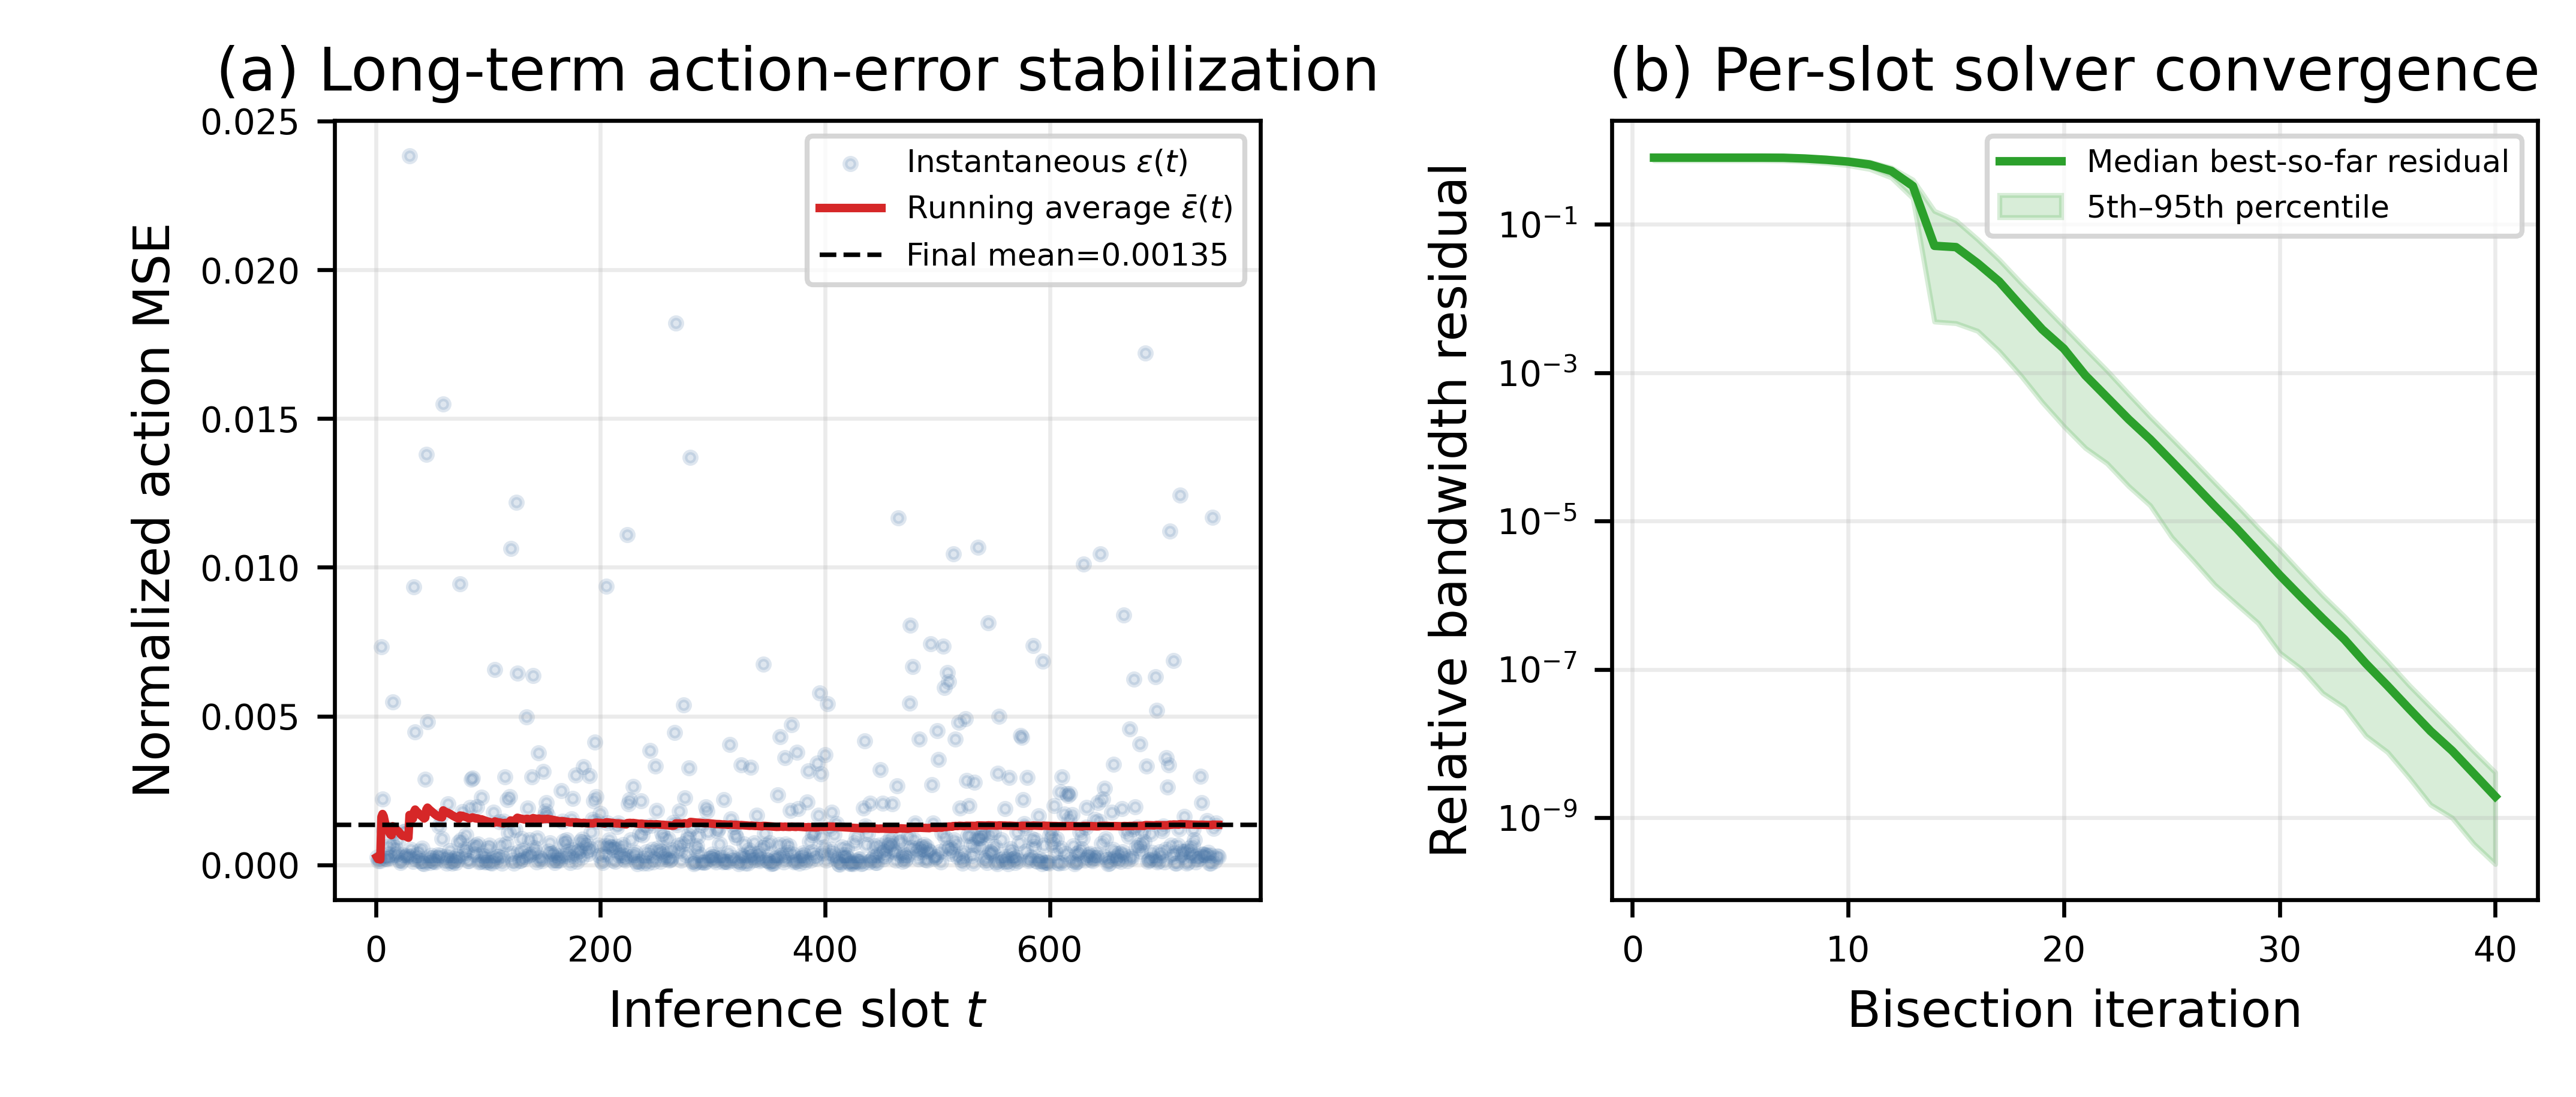
\includegraphics[width=0.95\linewidth]{convergence.png}
    \caption{Convergence of the proposed allocation scheme. (a) Running average of normalized action MSE over 750 inference slots, where the shaded area indicates the $95\%$ confidence interval. (b) Median best-so-far bandwidth residual versus bisection iterations.}
    \label{fig:convergence}
\end{figure}

\emph{2) Delayed relevance- and channel-aware adaptation:}
Fig.~\ref{fig:dynamic_allocation} demonstrates how the proposed
scheme converts delayed action relevance and instantaneous channel
quality into view-specific token allocations. At $t=0$, no historical
relevance is available and the predictor is initialized uniformly.
Nevertheless, the calibrated camera-specific parameters
$\{\beta_s,\gamma_s\}$ and heterogeneous transmission costs produce
the nonuniform allocation $(29,30,55)$ for
(\emph{side0}, \emph{side1}, \emph{wrist0}), showing the effect of the
offline marginal-utility calibration.

After the feedback warm-up, the three lower panels jointly illustrate
the adaptation mechanism. At $t=4$, the predicted relevance vector is
$(0.195,0.291,0.514)$ and the corresponding SNRs are
$(3.36,10.85,10.89)$~dB, resulting in the allocation $(12,35,70)$.
At $t=6$, the relevance of \emph{wrist0} increases to $0.628$ and its
SNR improves to $13.72$~dB; consequently, it receives all 81 tokens.
In contrast, the relevance of \emph{side0} decreases to $0.093$ while
its channel remains unfavorable at $3.98$~dB, reducing its allocation
to 10 tokens. At $t=9$, changes in both relevance and channel quality
lead to a new allocation of $(15,36,74)$. These examples confirm that
the proposed scheme does not allocate tokens according to relevance
or channel quality alone, but jointly balances the two factors through
(17).

The original--pruned observation pairs in the upper rows provide
visual evidence consistent with the resulting allocations. For
example, at $t=6$, the \emph{wrist0} observation, which exhibits the
largest predicted action relevance and a favorable channel condition,
is fully retained. In comparison, the \emph{side1} view is partially
retained, whereas most patches in the less relevant and
channel-disadvantaged \emph{side0} view are discarded. Together with
the relevance, SNR, and token-allocation trajectories in the lower
panels, these results illustrate that the proposed method dynamically
balances action relevance and wireless transmission cost rather than
allocating tokens according to either factor alone.

\begin{figure*}[t]
    \centering
    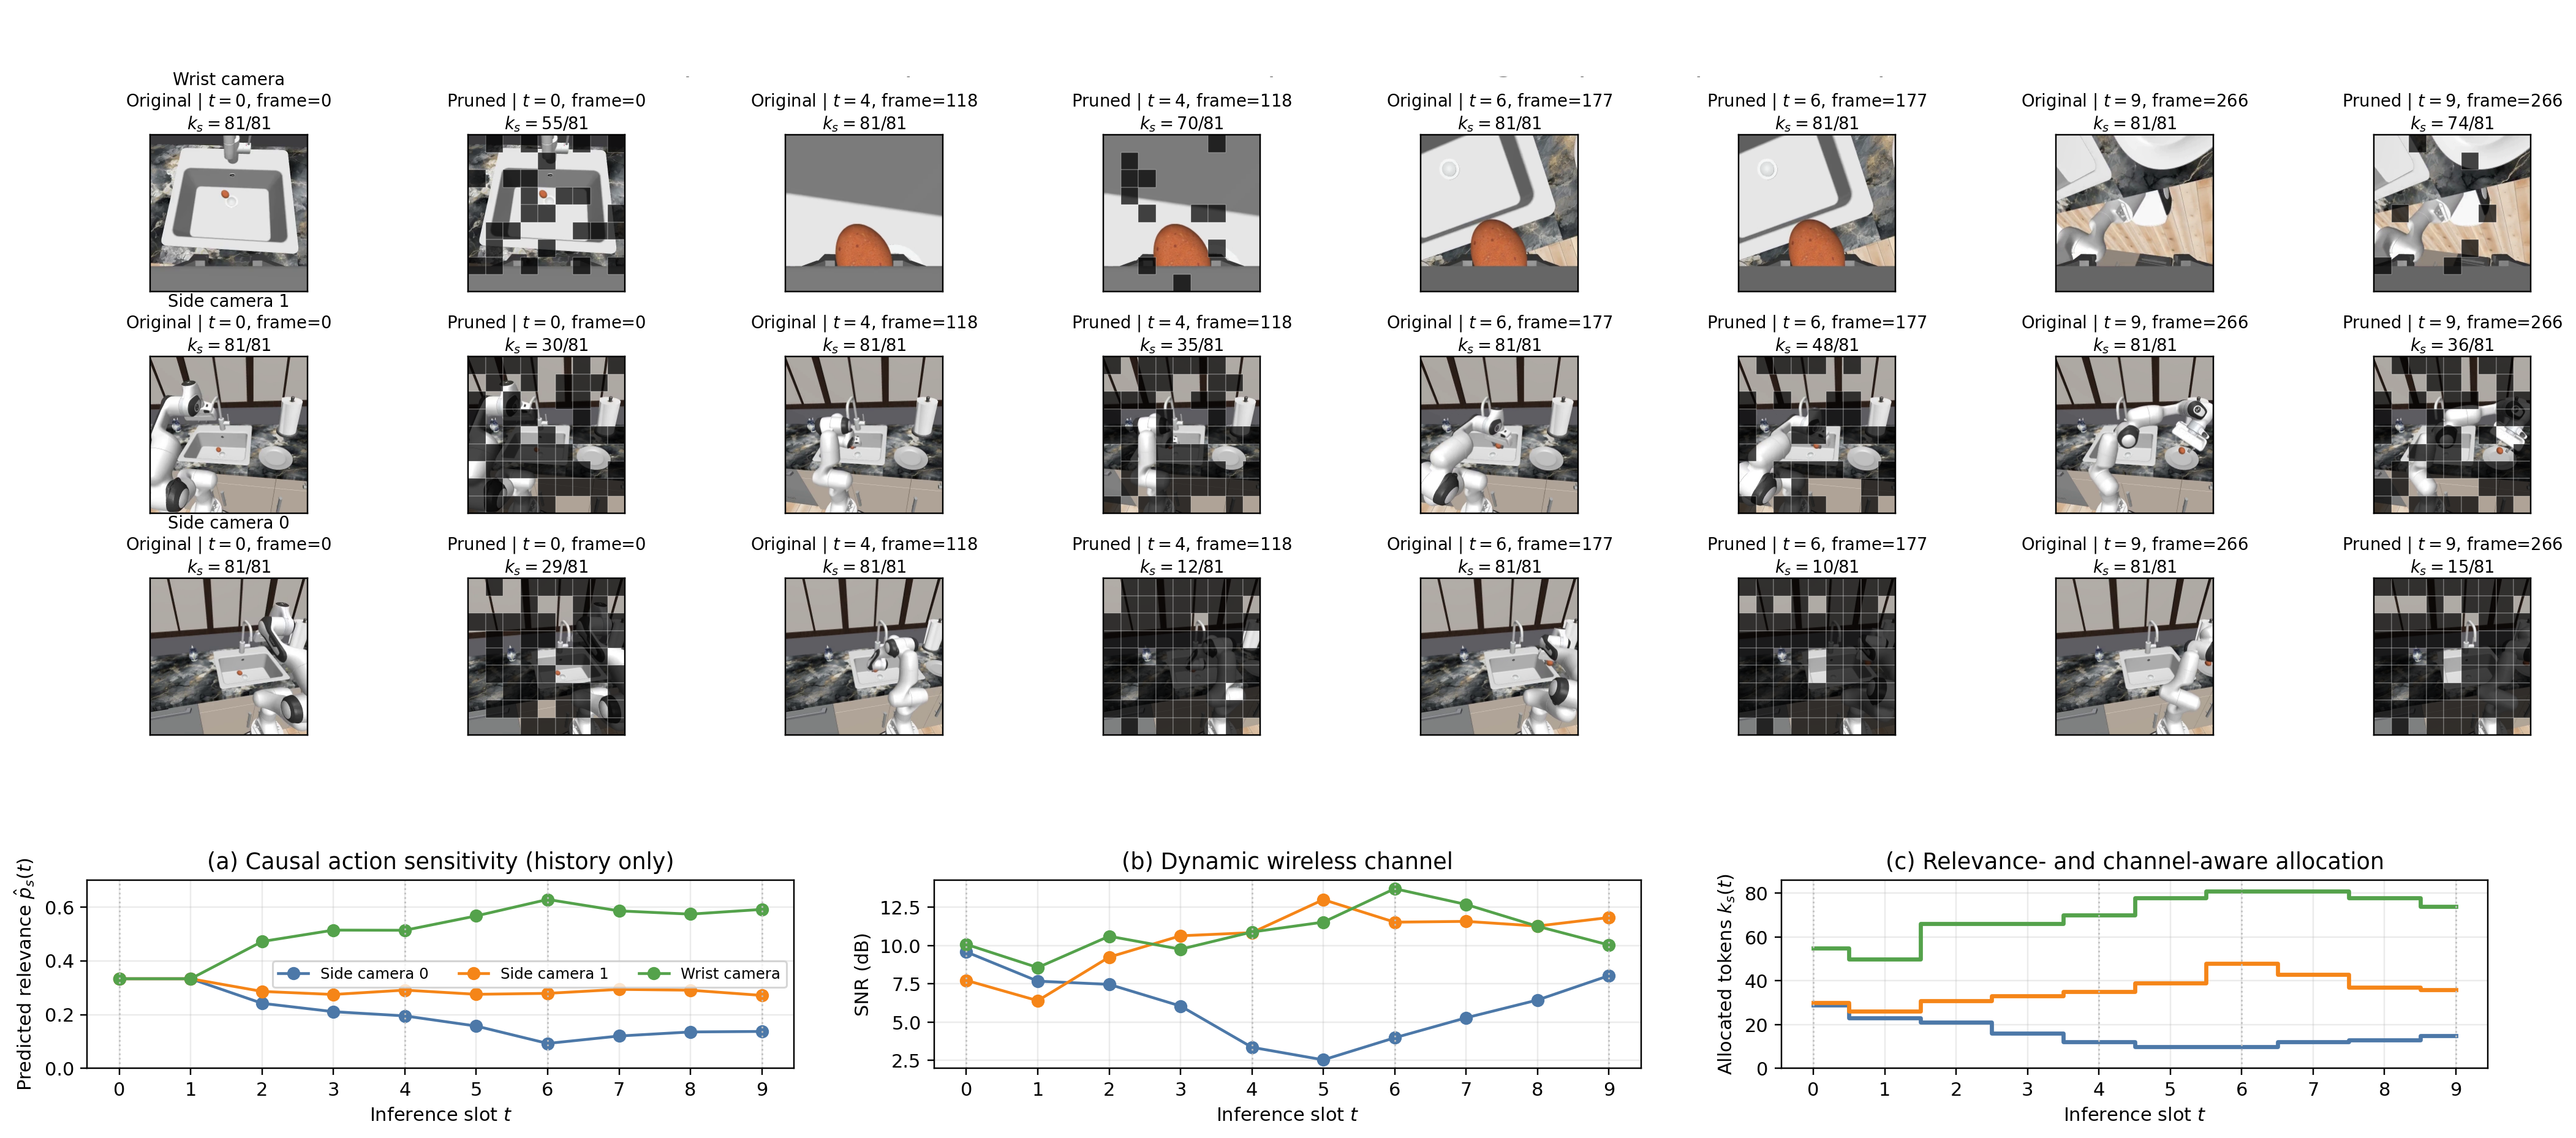
\includegraphics[width=0.95\textwidth]{dynamic_allocation.png}
    \caption{Dynamic token allocation under time-varying relevance and channel conditions. (Upper rows) Original (left) and pruned (right) observations for the three camera views, where black patches indicate discarded tokens. (Lower panels) Predicted view relevance $\widehat{p}_s(t)$, instantaneous SNR $\Gamma_s(t)$, and the resulting token allocation $k_s(t)$ over time.}
    \label{fig:dynamic_allocation}
\end{figure*}

\subsection{Impact of System Parameters}

Fig.~\ref{fig:snr_comparison} investigates the impact of the
nominal mean SNR $\bar{\Gamma}$ under the same $20$~MHz bandwidth
budget. As $\bar{\Gamma}$ increases from 12 to 20~dB, the per-token
transmission cost in (8) decreases, allowing more visual tokens to be
delivered within each control slot. Accordingly, the average number
of tokens retained by the proposed scheme increases from 148.95 to
207.24, while its normalized action MSE decreases from
$5.29\times10^{-4}$ to $8.98\times10^{-5}$, corresponding to an
approximately 83.0\% reduction. This result shows that the proposed
scheme effectively converts improved wireless channel quality into
better preservation of the full-token VLA action.

\begin{figure}[t]
    \centering
    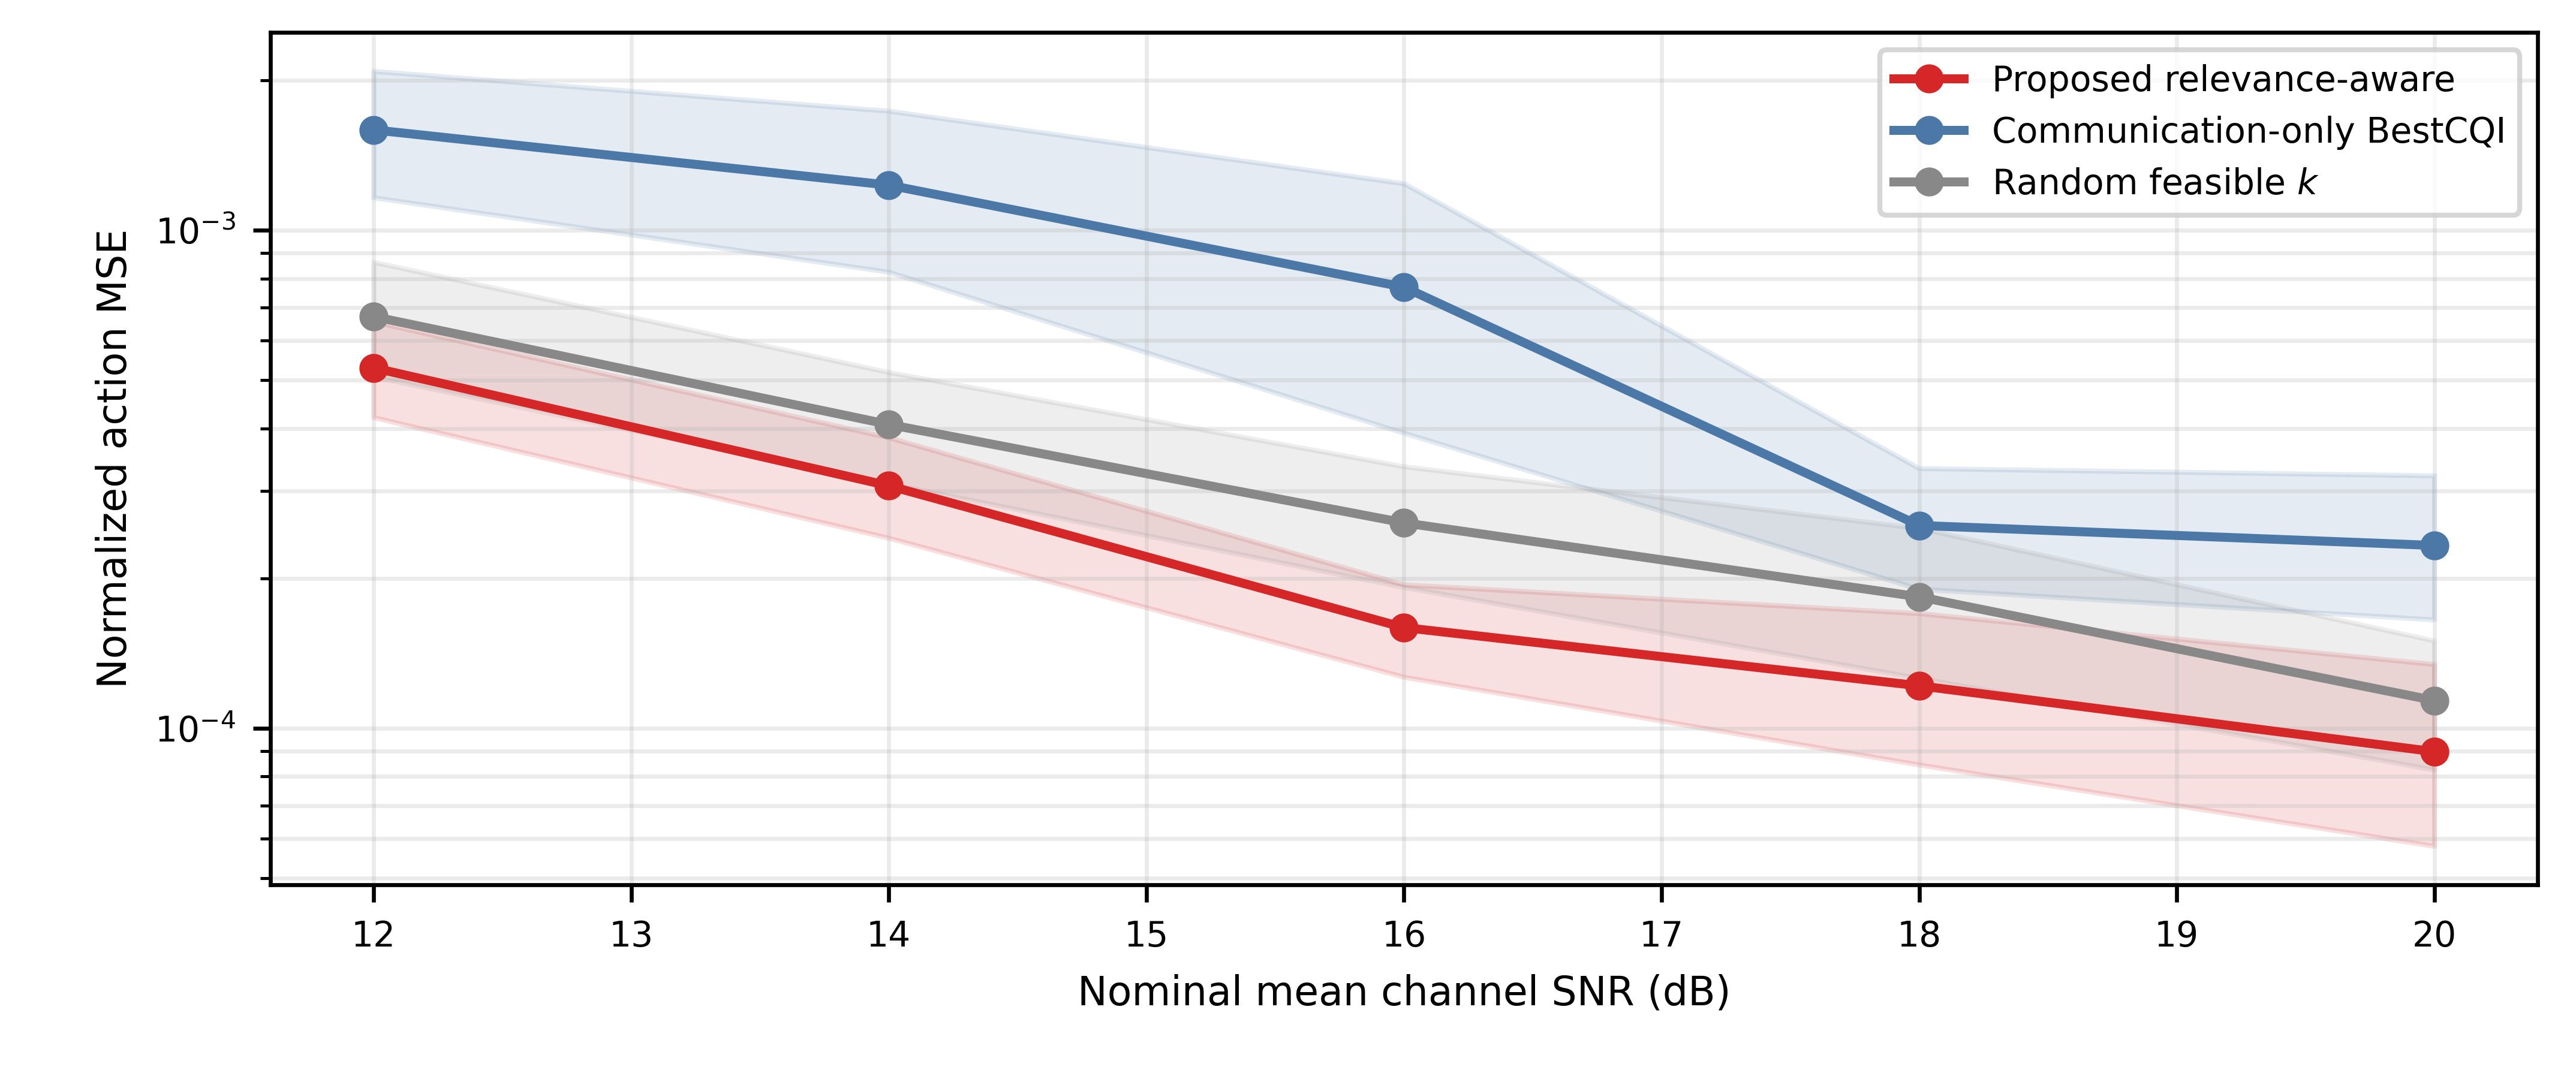
\includegraphics[width=\linewidth]{fig3_bestcqi_random_12_20db.png}
    \caption{Normalized VLA action MSE versus the nominal mean SNR $\bar{\Gamma}$ for the proposed scheme, BestCQI, and random allocation under the $20$~MHz bandwidth budget.}
    \label{fig:snr_comparison}
\end{figure}

Under the same channel realizations and bandwidth budget, the proposed
scheme achieves a lower mean action MSE than both baselines at every
evaluated SNR. Compared with BestCQI, it reduces the action MSE by
52.3\%--79.3\% across the five SNR points, with the paired 95\%
confidence intervals of the differences excluding zero in all cases.
Averaged over the complete SNR range, the reductions relative to
BestCQI and random feasible allocation are 70.4\% and 26.1\%,
respectively. The improvement over BestCQI demonstrates that allocating
tokens solely according to channel quality may favor views that are
inexpensive to transmit but less relevant to the current robot action.
By jointly considering action relevance and wireless transmission
cost, the proposed scheme uses the available bandwidth more effectively
to preserve VLA action performance.

\section{Conclusions}

This paper proposed an action-relevance-aware multi-view token
allocation scheme for wireless edge VLA inference. A
dataset-calibrated marginal action-utility model was established to
connect view-specific token allocation with VLA action preservation,
and a causal allocation method based on delayed relevance feedback
was developed. The resulting problem was solved using a generalized
water-filling method with integer-feasible correction. Experiments
with GR00T-N1.6-3B on the RoboCasa \emph{PnPSinkToCounter} task
demonstrated stable online allocation and rapid numerical convergence
under time-varying wireless channels. Across the evaluated SNR range,
the proposed scheme reduced the normalized action MSE by
52.3\%--79.3\% relative to BestCQI and by 26.1\% on average relative
to random feasible allocation. Future work will investigate online
recalibration across different tasks and sensor configurations and
evaluate the proposed method using closed-loop task-success metrics
in real wireless robotic systems.

\appendices
\section{Approximate Equivalence Between Problems~\ref{prob:p1} and~\ref{prob:p2}}\label{app:equivalence}
This appendix justifies Lemma~\ref{lem:marginal_law}. The sensor-specific marginal action-utility law and its parameters $\{\beta_s,\gamma_s\}$ are obtained independently by the offline calibration procedure in Appendix~\ref{app:calibration}. Under the calibration conditions stated therein, write the fitted marginal law as
\begin{align}\label{eq:app_marginal_residual}
    \mathbb E_{\mathcal D}\!\left[
    -\frac{\Delta\epsilon_{\bf k}}{\Delta k_s}
    \Bigm|p_s,k_s\right]
    =\beta_s\frac{p_s}{(k_s+1)^{\gamma_s}}+\xi_s(k_s,p_s),
\end{align}
where $\xi_s$ is the calibration residual. Neglecting $\xi_s$ and integrating the fitted marginal gain with respect to $k_s$ yields
\begin{align}
    U_s(k_s;p_s)=
    \begin{cases}
    \displaystyle\frac{\beta_s p_s}{1-\gamma_s}
    \left[(k_s+1)^{1-\gamma_s}-1\right], & \gamma_s\neq1,\\[1.5mm]
    \displaystyle\beta_s p_s\log(k_s+1), & \gamma_s=1,
    \end{cases}
\end{align}
which is exactly the utility in \eqref{eq:utility}. Under the separable marginal approximation across sensors, summing the integrated contributions gives
\begin{align}\label{eq:app_error_surrogate}
    \mathbb E_{\mathcal D}[\epsilon_{\bf k}\mid{\bf p}]
    \simeq C({\bf p})-\sum_{s\in\mathcal S}U_s(k_s;p_s),
\end{align}
where $C({\bf p})$ is independent of ${\bf k}$. Therefore, minimizing the dataset-averaged action error in Problem~\ref{prob:p1} is approximately equivalent to maximizing the sum utility in Problem~\ref{prob:p2}. Note that the elimination of $\{B_s(t)\}$ through \eqref{eq:reduced_bandwidth} is exact; only the objective transformation in \eqref{eq:app_error_surrogate} is empirical and approximate.

To quantify the approximation, suppose that the calibration residual in \eqref{eq:app_marginal_residual} is uniformly bounded over the deployment token range as $|\xi_s(k_s,p_s)|\leq\delta_s$. Accumulating the marginal residual then gives
\begin{align}
    \left|\Delta\epsilon_s-\Delta\widetilde\epsilon_s\right|
    \leq \delta_s\left(n_s-k_s^{\min}\right),
\end{align}
which provides a dataset-dependent bound on the objective mismatch induced by the fitted marginal model.

\section{Offline Calibration of the Sensor-Specific Marginal Utility Law}\label{app:calibration}
This appendix describes how the dataset-level parameters $\{\beta_s,\gamma_s\}$ used in Lemma~\ref{lem:marginal_law} and Appendix~\ref{app:equivalence} are obtained. Calibration is performed once during system preparation and introduces no online model training or parameter fitting.

\subsection{Calibration Assumptions}
The calibration is valid for a target dataset $\mathcal D$ under the following conditions: (i) the number, identity, intrinsics, extrinsics, and nominal placement of all sensors are unchanged between calibration and deployment; (ii) the same VLA checkpoint, visual tokenizer, token-pruning mechanism, and action normalization are used; (iii) calibration and deployment episodes are sampled from the same task/data distribution; and (iv) the tested token range covers the token budgets expected during deployment. If these conditions are violated, $\beta_s$ and $\gamma_s$ should be recalibrated.

\subsection{Counterfactual Marginal-Gain Sampling}
Let $\mathcal D_{\rm cal}\subset\mathcal D$ be a calibration subset that is disjoint from the final test episodes. For a sampled state $z$ and sensor $s$, we first perform a reference full-token VLA forward pass to obtain the view relevance $p_s(z)$. This relevance is frozen during the following counterfactual sweep. We then vary only the retained token number of sensor $s$ over a predefined grid $\mathcal K_s=\{k_{s,1},\ldots,k_{s,L}\}$ while keeping the other experimental settings fixed. For two adjacent token numbers, define the finite-difference marginal action gain as
\begin{align}\label{eq:cal_marginal}
    y_{s,i}(z)
    =\frac{\epsilon_{s,k_{s,i}}(z)-\epsilon_{s,k_{s,i+1}}(z)}
    {k_{s,i+1}-k_{s,i}},
\end{align}
which approximates $-\Delta\epsilon/\Delta k_s$. The action error is computed using the same reference-action definition as in Problem~\ref{prob:p1}. To suppress state-dependent VLA noise, samples are grouped into calibration-defined bins and the bin-wise expected marginal gain is used for fitting.

\subsection{Parameter Estimation}
For sensor $s$, the calibration model is
\begin{align}\label{eq:cal_fit}
    \bar y_{s,i}
    =\beta_s\frac{\bar p_{s,i}}{(\bar k_{s,i}+1)^{\gamma_s}}+\xi_{s,i},
\end{align}
where $\xi_{s,i}$ is the residual. We estimate the sensor-specific parameters by nonlinear least squares,
\begin{align}\label{eq:cal_nls}
    (\beta_s^\star,\gamma_s^\star)
    =\arg\min_{\beta_s>0,\gamma_s>0}
    \sum_i w_{s,i}
    \left(
    \bar y_{s,i}-
    \beta_s\frac{\bar p_{s,i}}{(\bar k_{s,i}+1)^{\gamma_s}}
    \right)^2,
\end{align}
where $w_{s,i}$ can be chosen as the number of samples in each bin or the inverse estimated variance of the bin mean. For any fixed $\gamma_s$, $\beta_s$ has the closed-form weighted least-squares solution
\begin{align}\label{eq:beta_closed}
    \beta_s^\star(\gamma_s)
    =\frac{\sum_i w_{s,i}x_{s,i}(\gamma_s)\bar y_{s,i}}
    {\sum_i w_{s,i}x_{s,i}^2(\gamma_s)},
\end{align}
where $x_{s,i}(\gamma_s)=\bar p_{s,i}/(\bar k_{s,i}+1)^{\gamma_s}$. Hence, only a one-dimensional search over $\gamma_s$ is required in practice.

\subsection{Example Calibrated Parameters}
For the fixed-sensor setting used in our numerical study, the offline calibration gives
\begin{align}
(\beta_s,\gamma_s)=
\begin{cases}
(0.005788,\ 1.333), & s=\mathrm{side0},\\
(0.01925,\ 1.623), & s=\mathrm{side1},\\
(0.6597,\ 2.322), & s=\mathrm{wrist0}.
\end{cases}\label{eq:fitted_params}
\end{align}
On 150 fresh independent test episodes, the corresponding $R^2$ values are $0.637$, $0.863$, and $0.930$, while the Pearson correlations are $0.798$, $0.930$, and $0.964$, respectively.

\subsection{Independent-Test Validation}
Fig.~\ref{fig:marginal_fit} shows the sensor-wise independent-test relationship used in this paper. The horizontal coordinate is $x_s=p_s/(k_s+1)^{\gamma_s}$ and the vertical coordinate is the binned expected marginal action gain. The fitted line is $\beta_s x_s$ with all parameters estimated only from the calibration split.
\begin{figure*}[t]
    \centering
    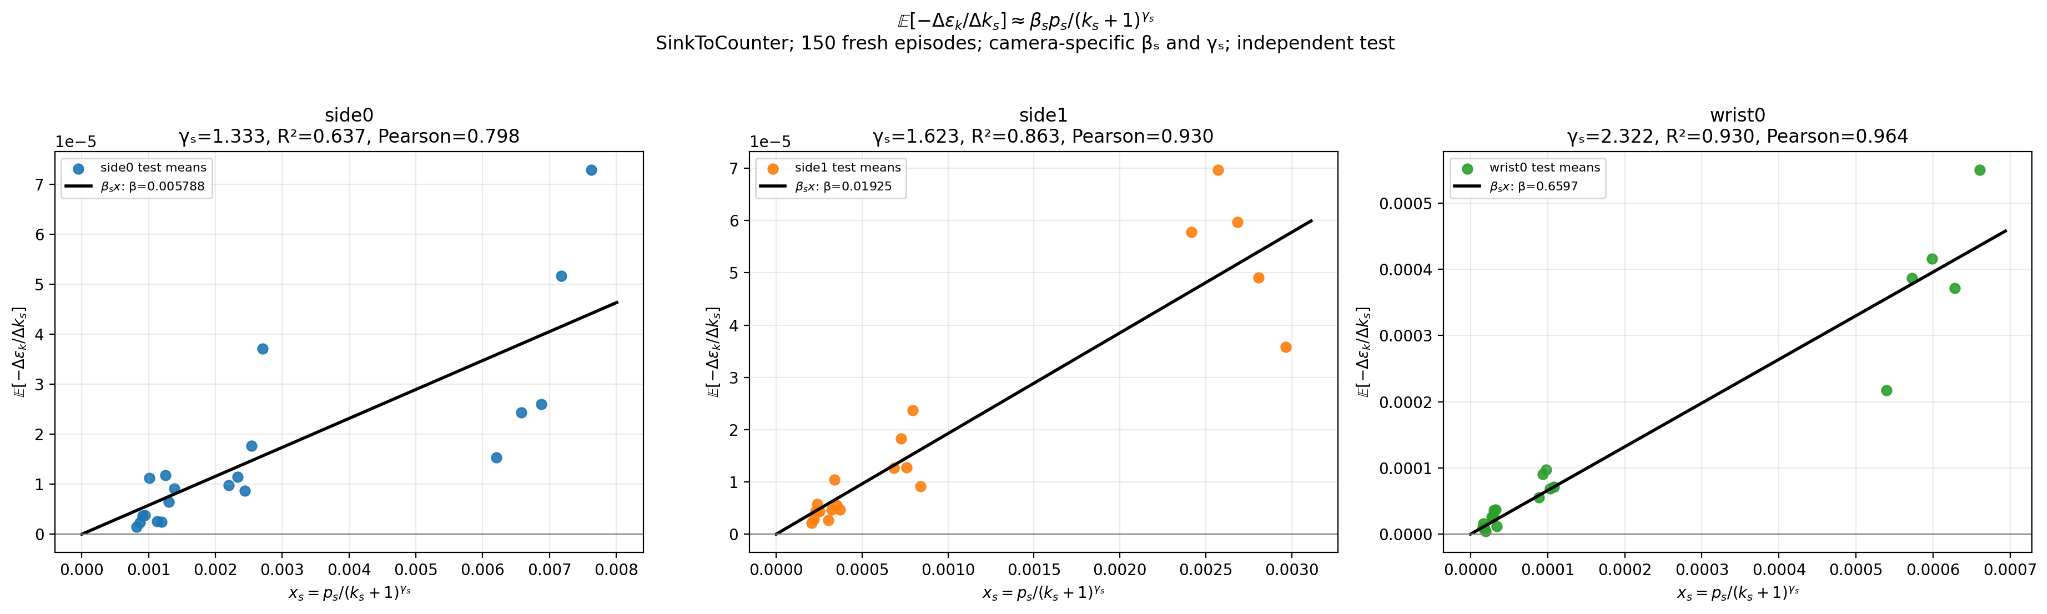
\includegraphics[width=0.98\textwidth]{marginal_utility_fit.png}
    \caption{Independent-test validation of the sensor-specific marginal action utility law on SinkToCounter. The sensor-specific $\beta_s$ and $\gamma_s$ are fitted on the calibration split and frozen before evaluation on 150 fresh episodes.}
    \label{fig:marginal_fit}
\end{figure*}
After calibration, $\beta_s^\star$ and $\gamma_s^\star$ are frozen and evaluated on fresh episodes that are not used for fitting. The validity of Lemma~\ref{lem:marginal_law} is assessed using the coefficient of determination $R^2$, Pearson correlation, Spearman rank correlation, and the residual error between the observed expected marginal gain and $\beta_s p_s/(k_s+1)^{\gamma_s}$. The resulting parameters are then stored as dataset-level constants and used by Algorithm~\ref{alg:allocation} throughout online execution.

\bibliographystyle{IEEEtranc}
\bibliography{IEEEfull, references, references_added} 



% \begin{thebibliography}{1}
% \bibliographystyle{IEEEtran}

% \bibitem{ref1}
% {\it{Mathematics Into Type}}. American Mathematical Society. [Online]. Available: https://www.ams.org/arc/styleguide/mit-2.pdf

% \bibitem{ref2}
% T. W. Chaundy, P. R. Barrett and C. Batey, {\it{The Printing of Mathematics}}. London, U.K., Oxford Univ. Press, 1954.

% \bibitem{ref3}
% F. Mittelbach and M. Goossens, {\it{The \LaTeX Companion}}, 2nd ed. Boston, MA, USA: Pearson, 2004.

% \bibitem{ref4}
% G. Gr\"atzer, {\it{More Math Into LaTeX}}, New York, NY, USA: Springer, 2007.

% \bibitem{ref5}M. Letourneau and J. W. Sharp, {\it{AMS-StyleGuide-online.pdf,}} American Mathematical Society, Providence, RI, USA, [Online]. Available: http://www.ams.org/arc/styleguide/index.html

% \bibitem{ref6}
% H. Sira-Ramirez, ``On the sliding mode control of nonlinear systems,'' \textit{Syst. Control Lett.}, vol. 19, pp. 303--312, 1992.

% \bibitem{ref7}
% A. Levant, ``Exact differentiation of signals with unbounded higher derivatives,''  in \textit{Proc. 45th IEEE Conf. Decis.
% Control}, San Diego, CA, USA, 2006, pp. 5585--5590. DOI: 10.1109/CDC.2006.377165.

% \bibitem{ref8}
% M. Fliess, C. Join, and H. Sira-Ramirez, ``Non-linear estimation is easy,'' \textit{Int. J. Model., Ident. Control}, vol. 4, no. 1, pp. 12--27, 2008.

% \bibitem{ref9}
% R. Ortega, A. Astolfi, G. Bastin, and H. Rodriguez, ``Stabilization of food-chain systems using a port-controlled Hamiltonian description,'' in \textit{Proc. Amer. Control Conf.}, Chicago, IL, USA,
% 2000, pp. 2245--2249.

% \end{thebibliography}


% \newpage

% \section{Biography Section}
% If you have an EPS/PDF photo (graphicx package needed), extra braces are
%  needed around the contents of the optional argument to biography to prevent
%  the LaTeX parser from getting confused when it sees the complicated
%  $\backslash${\tt{includegraphics}} command within an optional argument. (You can create
%  your own custom macro containing the $\backslash${\tt{includegraphics}} command to make things
%  simpler here.)
 
% \vspace{11pt}

% \bf{If you include a photo:}\vspace{-33pt}
% \begin{IEEEbiography}[{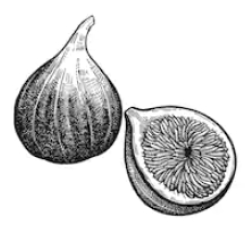
\includegraphics[width=1in,height=1.25in,clip,keepaspectratio]{fig1}}]{Michael Shell}
% Use $\backslash${\tt{begin\{IEEEbiography\}}} and then for the 1st argument use $\backslash${\tt{includegraphics}} to declare and link the author photo.
% Use the author name as the 3rd argument followed by the biography text.
% \end{IEEEbiography}

% \vspace{11pt}

% \bf{If you will not include a photo:}\vspace{-33pt}
% \begin{IEEEbiographynophoto}{John Doe}
% Use $\backslash${\tt{begin\{IEEEbiographynophoto\}}} and the author name as the argument followed by the biography text.
% \end{IEEEbiographynophoto}




\vfill

\end{document}


